
\documentclass[letterpaper,hide notes,xcolor={table,svgnames},pdftex,10pt]{beamer}
\def\showexamples{t}


%\usepackage[svgnames]{xcolor}

%% Demo talk
%\documentclass[letterpaper,notes=show]{beamer}

\usecolortheme{crane}
\setbeamertemplate{navigation symbols}{}

\usetheme{MyPittsburgh}
%\usetheme{Frankfurt}

%\usepackage{tipa}

\usepackage{hyperref}
\usepackage{graphicx,xspace}
\usepackage[normalem]{ulem}
\usepackage{multicol}
\usepackage{amsmath,amssymb,amsthm,graphicx,xspace}
\newcommand\SF[1]{$\bigstar$\footnote{SF: #1}}

\usepackage[default]{sourcesanspro}
\usepackage[T1]{fontenc}
\usepackage[scaled]{beramono}
\usepackage{tikzpagenodes}

\newcounter{tmpnumSlide}
\newcounter{tmpnumNote}


% old question code
%\newcommand\question[1]{{$\bigstar$ \small \onlySlide{2}{#1}}}
% \newcommand\nquestion[1]{\ifdefined \presentationonly \textcircled{?} \fi \note{\par{\Large \textbf{?}} #1}}
% \newcommand\nanswer[1]{\note{\par{\Large \textbf{A}} #1}}


 \newcommand\mnote[1]{%
   \addtocounter{tmpnumSlide}{1}
   \ifdefined\showcues {~\tiny\fbox{\arabic{tmpnumSlide}}}\fi
   \note{\setlength{\parskip}{1ex}\addtocounter{tmpnumNote}{1}\textbf{\Large \arabic{tmpnumNote}:} {#1\par}}}

\newcommand\mmnote[1]{\note{\setlength{\parskip}{1ex}#1\par}}

%\newcommand\mnote[2][]{\ifdefined\handoutwithnotes {~\tiny\fbox{#1}}\fi
% \note{\setlength{\parskip}{1ex}\textbf{\Large #1:} #2\par}}

%\newcommand\mnote[2][]{{\tiny\fbox{#1}} \note{\setlength{\parskip}{1ex}\textbf{\Large #1:} #2\par}}

\newcommand\mquestion[2]{{~\color{red}\fbox{?}}\note{\setlength{\parskip}{1ex}\par{\Large \textbf{?}} #1} \note{\setlength{\parskip}{1ex}\par{\Large \textbf{A}} #2\par}\ifdefined \presentationonly \pause \fi}

\newcommand\blackboard[1]{%
\ifdefined   \showblackboard
  {#1}
  \else {\begin{center} \fbox{\colorbox{blue!30}{%
         \begin{minipage}{.95\linewidth}%
           \hspace{\stretch{1}} Some space intentionally left blank; done at the blackboard.%
         \end{minipage}}}\end{center}}%
         \fi%
}



%\newcommand\q{\tikz \node[thick,color=black,shape=circle]{?};}
%\newcommand\q{\ifdefined \presentationonly \textcircled{?} \fi}

\usepackage{listings}
\lstset{basicstyle=\footnotesize\ttfamily,
	breaklines=true,
	aboveskip=15pt,
  	belowskip=15pt,
	frame=lines,
	numbers=left, basicstyle=\scriptsize, numberstyle=\tiny, stepnumber=0, numbersep=2pt
}

\usepackage{siunitx}
\newcommand\sius[1]{\num[group-separator = {,}]{#1}\si{\micro\second}}
\newcommand\sims[1]{\num[group-separator = {,}]{#1}\si{\milli\second}}
\newcommand\sins[1]{\num[group-separator = {,}]{#1}\si{\nano\second}}
\sisetup{group-separator = {,}, group-digits = true}

%% -------------------- tikz --------------------
\usepackage{tikz}
\usetikzlibrary{positioning}
\usetikzlibrary{arrows,backgrounds,automata,decorations.shapes,decorations.pathmorphing,decorations.markings,decorations.text,decorations.pathreplacing}

\tikzstyle{place}=[circle,draw=blue!50,fill=blue!20,thick, inner sep=0pt,minimum size=6mm]
\tikzstyle{transition}=[rectangle,draw=black!50,fill=black!20,thick, inner sep=0pt,minimum size=4mm]

\tikzstyle{block}=[rectangle,draw=black, thick, inner sep=5pt]
\tikzstyle{bullet}=[circle,draw=black, fill=black, thin, inner sep=2pt]

\tikzstyle{pre}=[<-,shorten <=1pt,>=stealth',semithick]
\tikzstyle{post}=[->,shorten >=1pt,>=stealth',semithick]
\tikzstyle{bi}=[<->,shorten >=1pt,shorten <=1pt, >=stealth',semithick]

\tikzstyle{mut}=[-,>=stealth',semithick]

\tikzstyle{treereset}=[dashed,->, shorten >=1pt,>=stealth',thin]

\usepackage{ifmtarg}
\usepackage{xifthen}
\makeatletter
% new counter to now which frame it is within the sequence
\newcounter{multiframecounter}
% initialize buffer for previously used frame title
\gdef\lastframetitle{\textit{undefined}}
% new environment for a multi-frame
\newenvironment{multiframe}[1][]{%
\ifthenelse{\isempty{#1}}{%
% if no frame title was set via optional parameter,
% only increase sequence counter by 1
\addtocounter{multiframecounter}{1}%
}{%
% new frame title has been provided, thus
% reset sequence counter to 1 and buffer frame title for later use
\setcounter{multiframecounter}{1}%
\gdef\lastframetitle{#1}%
}%
% start conventional frame environment and
% automatically set frame title followed by sequence counter
\begin{frame}%
\frametitle{\lastframetitle~{\normalfont(\arabic{multiframecounter})}}%
}{%
\end{frame}%
}
\makeatother

\makeatletter
\newdimen\tu@tmpa%
\newdimen\ydiffl%
\newdimen\xdiffl%
\newcommand\ydiff[2]{%
    \coordinate (tmpnamea) at (#1);%
    \coordinate (tmpnameb) at (#2);%
    \pgfextracty{\tu@tmpa}{\pgfpointanchor{tmpnamea}{center}}%
    \pgfextracty{\ydiffl}{\pgfpointanchor{tmpnameb}{center}}%
    \advance\ydiffl by -\tu@tmpa%
}
\newcommand\xdiff[2]{%
    \coordinate (tmpnamea) at (#1);%
    \coordinate (tmpnameb) at (#2);%
    \pgfextractx{\tu@tmpa}{\pgfpointanchor{tmpnamea}{center}}%
    \pgfextractx{\xdiffl}{\pgfpointanchor{tmpnameb}{center}}%
    \advance\xdiffl by -\tu@tmpa%
}
\makeatother
\newcommand{\copyrightbox}[3][r]{%
\begin{tikzpicture}%
\node[inner sep=0pt,minimum size=2em](ciimage){#2};
\usefont{OT1}{phv}{n}{n}\fontsize{4}{4}\selectfont
\ydiff{ciimage.south}{ciimage.north}
\xdiff{ciimage.west}{ciimage.east}
\ifthenelse{\equal{#1}{r}}{%
\node[inner sep=0pt,right=1ex of ciimage.south east,anchor=north west,rotate=90]%
{\raggedleft\color{black!50}\parbox{\the\ydiffl}{\raggedright{}#3}};%
}{%
\ifthenelse{\equal{#1}{l}}{%
\node[inner sep=0pt,right=1ex of ciimage.south west,anchor=south west,rotate=90]%
{\raggedleft\color{black!50}\parbox{\the\ydiffl}{\raggedright{}#3}};%
}{%
\node[inner sep=0pt,below=1ex of ciimage.south west,anchor=north west]%
{\raggedleft\color{black!50}\parbox{\the\xdiffl}{\raggedright{}#3}};%
}
}
\end{tikzpicture}
}


%% --------------------

%\usepackage[excludeor]{everyhook}
%\PushPreHook{par}{\setbox0=\lastbox\llap{MUH}}\box0}

%\vspace*{\stretch{1}

%\setbox0=\lastbox \llap{\textbullet\enskip}\box0}

\setlength{\parskip}{\fill}

\newcommand\noskips{\setlength{\parskip}{1ex}}
\newcommand\doskips{\setlength{\parskip}{\fill}}

\newcommand\xx{\par\vspace*{\stretch{1}}\par}
\newcommand\xxs{\par\vspace*{2ex}\par}
\newcommand\tuple[1]{\langle #1 \rangle}
\newcommand\code[1]{{\sf \footnotesize #1}}
\newcommand\ex[1]{\uline{Example:} \ifdefined \presentationonly \pause \fi
  \ifdefined\showexamples#1\xspace\else{\uline{\hspace*{2cm}}}\fi}

\newcommand\ceil[1]{\lceil #1 \rceil}


\AtBeginSection[]
{
   \begin{frame}
       \frametitle{Outline}
       \tableofcontents[currentsection]
   \end{frame}
}



\pgfdeclarelayer{edgelayer}
\pgfdeclarelayer{nodelayer}
\pgfsetlayers{edgelayer,nodelayer,main}

\tikzstyle{none}=[inner sep=0pt]
\tikzstyle{rn}=[circle,fill=Red,draw=Black,line width=0.8 pt]
\tikzstyle{gn}=[circle,fill=Lime,draw=Black,line width=0.8 pt]
\tikzstyle{yn}=[circle,fill=Yellow,draw=Black,line width=0.8 pt]
\tikzstyle{empty}=[circle,fill=White,draw=Black]
\tikzstyle{bw} = [rectangle, draw, fill=blue!20, 
    text width=4em, text centered, rounded corners, minimum height=2em]
    
    \newcommand{\CcNote}[1]{% longname
	This work is licensed under the \textit{Creative Commons #1 3.0 License}.%
}
\newcommand{\CcImageBy}[1]{%
	\includegraphics[scale=#1]{creative_commons/cc_by_30.pdf}%
}
\newcommand{\CcImageSa}[1]{%
	\includegraphics[scale=#1]{creative_commons/cc_sa_30.pdf}%
}
\newcommand{\CcImageNc}[1]{%
	\includegraphics[scale=#1]{creative_commons/cc_nc_30.pdf}%
}
\newcommand{\CcGroupBySa}[2]{% zoom, gap
	\CcImageBy{#1}\hspace*{#2}\CcImageNc{#1}\hspace*{#2}\CcImageSa{#1}%
}
\newcommand{\CcLongnameByNcSa}{Attribution-NonCommercial-ShareAlike}

\newenvironment{changemargin}[1]{% 
  \begin{list}{}{% 
    \setlength{\topsep}{0pt}% 
    \setlength{\leftmargin}{#1}% 
    \setlength{\rightmargin}{1em}
    \setlength{\listparindent}{\parindent}% 
    \setlength{\itemindent}{\parindent}% 
    \setlength{\parsep}{\parskip}% 
  }% 
  \item[]}{\end{list}} 




\title{Lecture 34 --- DevOps for P4P }

\author{Patrick Lam \& Jeff Zarnett \\ \small \texttt{patrick.lam@uwaterloo.ca} \texttt{jzarnett@uwaterloo.ca}}
\institute{Department of Electrical and Computer Engineering \\
  University of Waterloo}
\date{\today}


\begin{document}

\begin{frame}
  \titlepage

 \end{frame}



\begin{frame}
\frametitle{DevOps for P4P}

\Large
\begin{changemargin}{2cm}
So far, one-off computations:\\
you need to answer a question, \\
so you write code to
do that.\\[1em]
But many systems are long-running.\\[1em]
$\Rightarrow$ Operations.
\end{changemargin}

\end{frame}



\begin{frame}
\frametitle{Keep it Rolling}

\Large
\begin{changemargin}{1cm}
MPI: still mostly one-off computations\\
(even though on multiple computers.)\\[1em]
Cloud computing: often long-lived systems,\\
but we didn't talk about how.\\[1em]
Today: many companies fuse\\
development (writes the software) \\
and operations (tends the software).
\end{changemargin}
\end{frame}



\begin{frame}
\frametitle{Disaster Girl Strikes Again}

\begin{center}
	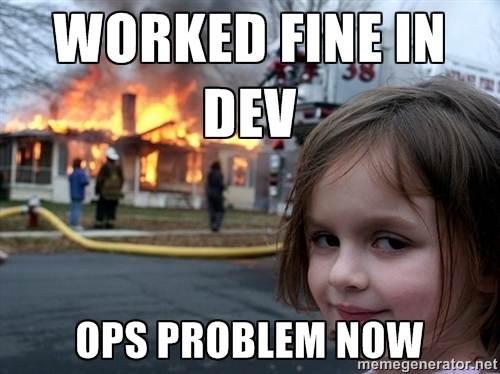
\includegraphics[width=0.8\textwidth]{images/devops.jpg}
\end{center}

\end{frame}



\begin{frame}
\frametitle{Start Me Up}

\Large
\begin{changemargin}{1cm}
Startups:\\[1em]
No money to pay for separate \\
developer and operations teams.\\[1em]
Not that many servers, \\
just a few demo systems, test systems, etc\ldots\\
but it spirals out from there. \\[1em]
You're not really going to ask Sales to manage these servers, are you? \\
So, there's DevOps. 
\end{changemargin}

\end{frame}



\begin{frame}
\frametitle{DevOps---Good Plan?}

\large
\begin{changemargin}{1cm}
Is DevOps a good idea? \\
Can be used for both good and evil. \\[1em]
Good:
\begin{itemize}
\item developers involved across the software lifecycle.\\
(can learn a lot doing ops\ldots )
\item developers motivated to use correct tools \& document processes.
\end{itemize}
\end{changemargin}

\end{frame}



\begin{frame}
\frametitle{On the Other Hand...}

\large
\begin{changemargin}{1cm}
Ugly:
\begin{itemize}
\item also something to be said for \\
never letting the developers out of their cubes and \\
keeping them far, far away from  customers. \\\

They will be scared. \\

Both parties.
\end{itemize}
\end{changemargin}
\end{frame}



\begin{frame}
\frametitle{Configuration as Code}

\large
\begin{changemargin}{2cm}
Systems have long come with \\
complicated (``flexible'') configuration options.


Sendmail is particularly notorious, but apache and nginx aren't super
easy to configure either.

First principle: treat \emph{configuration as code}.
\end{changemargin}

\end{frame}



\begin{frame}
\frametitle{Configuration as Code}

\large
\begin{changemargin}{2cm}
\begin{itemize}
\item use version control on your configuration.
\item test your configurations.
\item aim for a suite of modular services that integrate together smoothly.
\item refactor configuration files.
\item use continuous builds (more on that later).
\end{itemize}
\end{changemargin}

\end{frame}



\begin{frame}
\frametitle{Autoconfig}

\large
\begin{changemargin}{2cm}
Excellent idea: tools for configuration. \\[1em]

Not enough to write text \\
\qquad ``How to Install AwesomeApp'' \\[1em]

e.g. use Red Hat Package Manager (RPM)---\\
build, installation, and update automatic \& simple.\\[1em]

 Complicated means mistakes\ldots people forget steps. They are human. 
 \end{changemargin}
 
\end{frame}



\begin{frame}
\frametitle{Servers as Cattle, not Pets}

\large
\begin{changemargin}{2cm}
Servers means servers, or virtual machines, or containers.\\[1em]

At scale (smaller than you think):\\
use mass tools for dealing with servers, \\
rather than doing tasks manually. \\[1em]

At least: cloud-like server initialization without manual intervention;\\
must be able to spin up a server programmatically.
\end{changemargin}

\end{frame}



\begin{frame}
\frametitle{Common Infrastructure}

\large
\begin{changemargin}{1cm}
Use APIs to access your infrastructure. Examples:

\begin{itemize}
\item storage: access layer to MongoDB/Amazon S3/etc;
\item naming and discovery infrastructure;
\item monitoring infrastructure.
\end{itemize}

Avoid one-offs---use open-source tools when applicable.\\
But build your own tools if needed.
\end{changemargin}

\end{frame}



\begin{frame}
\frametitle{Rule of Ten}

\large
\begin{changemargin}{1cm}
eBay:
\begin{itemize}
\item 1995: perl scripts;
\item 1997: C++/Windows;
\item 2002: Java.
\end{itemize}

Each of these architectures was appropriate at the time, \\
but not as requirements changed. \\[1em]

More sophisticated successor architectures \\
would have been overkill earlier.

Hard to predict what's needed in the future.
\end{changemargin}

\end{frame}



\begin{frame}
\frametitle{Perf}

\large
\begin{changemargin}{1cm}
\begin{quote}
``Perf is a feature''.\\
\hfill --- Jeff Atwood
\end{quote}
That is: apply developer time to perf, \\
and make engineering tradeoffs to get it.\\[1em]

Some thoughts:
\begin{itemize}
\item design with the eventual replacement in mind;
\item don't abandon internal quality (e.g. modularity);
\item sacrifice individual modules at a time,\\
not the whole system;
\item implement new features with a rough draft and deploy to a test audience.
\end{itemize}
\end{changemargin}


\end{frame}




\begin{frame}
\frametitle{Naming}

\Large
\begin{changemargin}{1cm}
Naming is one of the hard problems in computing. 

There are only two hard things in computers:
\begin{enumerate}
\item cache invalidation,
\item naming things, and
\item off by one errors.
\end{enumerate}
\end{changemargin}
\end{frame}



\begin{frame}
\frametitle{Naming Suggestions}

\large
\begin{changemargin}{1cm}
\begin{itemize}
\item use canonical one-word names for servers;
\item but, use aliases to specify functions, e.g. 1) geography (nyc); 2) environment (dev/tst/stg/prod); 
3) purpose (app/sql/etc); and 4) serial number.
\end{itemize}


There's also the Java package approach of infinite dots: live.application.customer.webdomain.com or however you want to call it. 

Pick something and be consistent.
\end{changemargin}
\end{frame}



\begin{frame}
\frametitle{Continuous Integration}

\Large
\begin{changemargin}{1cm}
\begin{itemize}
\item pull code from version control;
\item build;
\item run tests;
\item report results.
\end{itemize}

\end{changemargin}

\end{frame}

\begin{frame}
\frametitle{Continuous Integration Social Convention}

\Large
\begin{changemargin}{1cm}
Don't break the build (or donuts).
\end{changemargin}
\begin{center}
\includegraphics[width=.6\textwidth]{images/L35-dunkin-coffee.jpg}
\end{center}

\begin{changemargin}{1cm}
Run the CI cycle on every commit;\\
results sent by e-mail or instant messenger.
\end{changemargin}
\end{frame}

\begin{frame}
\frametitle{Canarying}

\begin{center}
	
\includegraphics[width=0.9\textwidth]{images/blackcanary.jpg}
\end{center}

\end{frame}



\begin{frame}
\frametitle{Canarying}

\large
\begin{changemargin}{1cm}
Deploy new code incrementally in production, \\
also known as ``test in prod'':


\begin{itemize}
\item stage for deployment;
\item remove canary servers from service;
\item upgrade canary servers;
\item run automatic tests on upgraded canaries;
\item reintroduce canary servers into service;
\item see how it goes!
\end{itemize}

Of course: implement your system with rollback.
\end{changemargin}

\end{frame}



\begin{frame}
\frametitle{Monitoring}
\large
\begin{changemargin}{1cm}
Things to think about:

\begin{itemize}
	\item CPU Load
	\item Memory Utilization
	\item Disk Space
	\item Disk I/O
	\item Network Traffic
	\item Clock Skew
	\item Application Response Times
\end{itemize}
\end{changemargin}

\end{frame}



\begin{frame}
\frametitle{Dashboard}

\large
\begin{changemargin}{1cm}
Multiple systems: need an overview of all the systems.\\[1em]

Summary needs to show whether anything is wrong, \\
but not an overwhelming wall of data.
\end{changemargin}
\end{frame}

{
\usebackgroundtemplate{
\includegraphics[height=\paperheight,width=\paperwidth]{images/L35-RedAlert.jpg}}
\begin{frame}[plain]

\end{frame}
}

\begin{frame}
\frametitle{Dashboard}

\large
\begin{changemargin}{1cm}

Don't pay someone to stare at the dashboard and\\
press the  ``Red Alert!'' button \\
if anything goes out of some preset range.

No, for that we need some automatic monitoring.
\end{changemargin}

\end{frame}



\begin{frame}
\frametitle{Red Alert}

\large
\begin{changemargin}{1cm}
\begin{itemize}
\item {\bf Alerts}: a human must take action now;
\item {\bf Tickets}: a human must take action soon \\ \qquad (hours or days);
\item {\bf Logging}: no need to look at this \\ \qquad except for forensic/diagnostic purposes.
\end{itemize}


Common bad situation: logs-as-tickets.
\end{changemargin}
\end{frame}



{
\usebackgroundtemplate{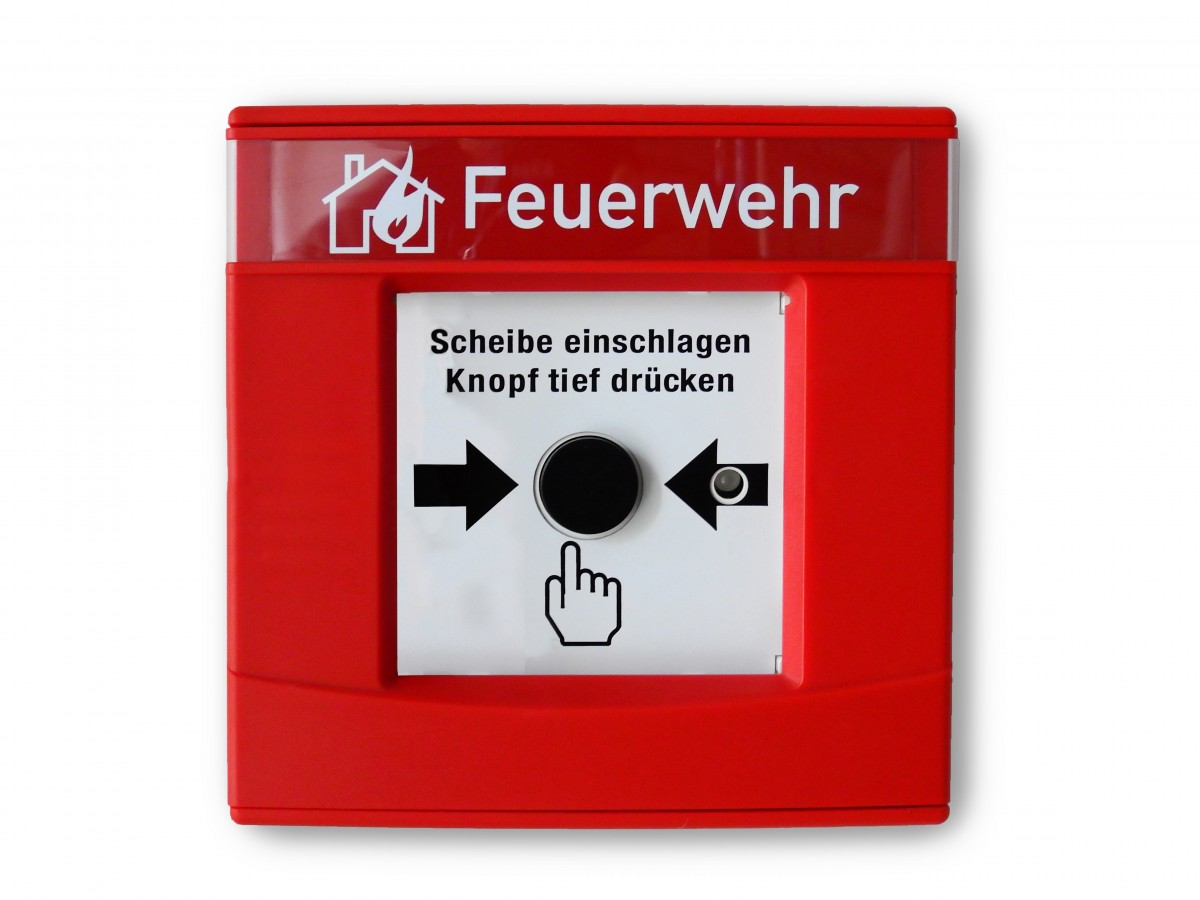
\includegraphics[height=\paperheight,width=\paperwidth]{images/L35-fire-alarm.jpg}}
\begin{frame}[plain]

\end{frame}
}

\begin{frame}
\frametitle{Action Stations! Set Condition One Throughout the Ship}

\large
\begin{changemargin}{1cm}
What do you do when you hear the fire alarm?\\[1em]
%% It is very important to be judicious about the use of alerts. 

%% If your alerts are too common, they get ignored. 

%% When you hear the fire alarm in a building, chances are your thought is not ``the building is on fire; I should leave it immediately in an orderly fashion.''.

%% It's a good heuristic; you'll be correct most of the time. 

If there is an actual fire, you will not only be wrong, \\
you might also be dead.
\end{changemargin}
\end{frame}



\begin{frame}
\frametitle{Not the Kittens!!!}

\large
\begin{changemargin}{1cm}
Alerts and tickets are a great way to make user pain into developer pain.

Some SUPER CRITICAL ticket OMG KITTENS ARE ENDANGERED is an excellent way to learn the lesson... 

Devs will take steps that keep these things from happening in the future.
\end{changemargin}
\end{frame}




\end{document}

